\chapter{系统需求分析与总体架构设计}
本章将详细介绍系统的功能需求分析和总体架构设计。首先,我们将深入分析系统需要满足的功能需求,涵盖自然语言输入、语义理解、场景生成、仿真执行以及多样场景支持等关键方面。这些功能需求将为系统的设计提供明确的方向和目标。接着,我们将阐述系统的总体架构设计,包括架构目标、设计原则、架构图展示以及模块间的数据流和交互机制。通过这些内容,读者可以对系统的整体设计有一个清晰的了解,为后续章节中各模块的具体设计与实现奠定基础。
\section{系统功能需求分析}
\subsection{高保真的驾驶测试需求}
随着自动驾驶技术的快速发展,自动驾驶系统的测试与验证变得尤为重要。传统的测试方法通常依赖于手动构建的场景,这种方法不仅耗时费力,而且难以覆盖复杂的交通场景。为了提高测试效率和覆盖度,本研究提出了一种基于自然语言描述的三维智能驾驶场景生成系统。该系统能够自动将用户输入的自然语言场景描述转化为可执行的仿真场景,并在CARLA仿真平台上进行验证。

本系统的核心优势之一是能够利用生成的智能驾驶场景,为自动驾驶技术提供一个高效、低成本的测试平台。传统的人工构建测试场景方法不仅耗时费力,而且难以覆盖复杂的交通场景,导致测试成本高昂且效率低下。相比之下,本系统通过自然语言输入和自动化场景生成技术,能够快速生成多样化的驾驶场景,显著提高了测试效率。用户只需通过简单的自然语言描述输入,系统即可自动生成对应的三维智能驾驶场景,并在 CARLA 仿真平台上进行验证。这种自动化流程大大减少了人工干预,降低了测试成本。此外,系统支持多种语义表达和场景组合,能够生成丰富的测试用例,满足不同阶段的自动驾驶技术测试需求。通过这种方式,本系统不仅能够加速智能驾驶技术的开发和验证过程,还能为研究人员和工程师提供一个灵活、可扩展的测试工具,推动智能驾驶技术的发展。


\section{系统总体架构设计}
系统整体采用模块化分层设计,主要分为三个核心模块,每个模块分有几个子模块分别负责不同阶段的处理任务,构成完整的自然语言驱动智能驾驶场景生成流程:
\begin{figure}[H]
	\centering
	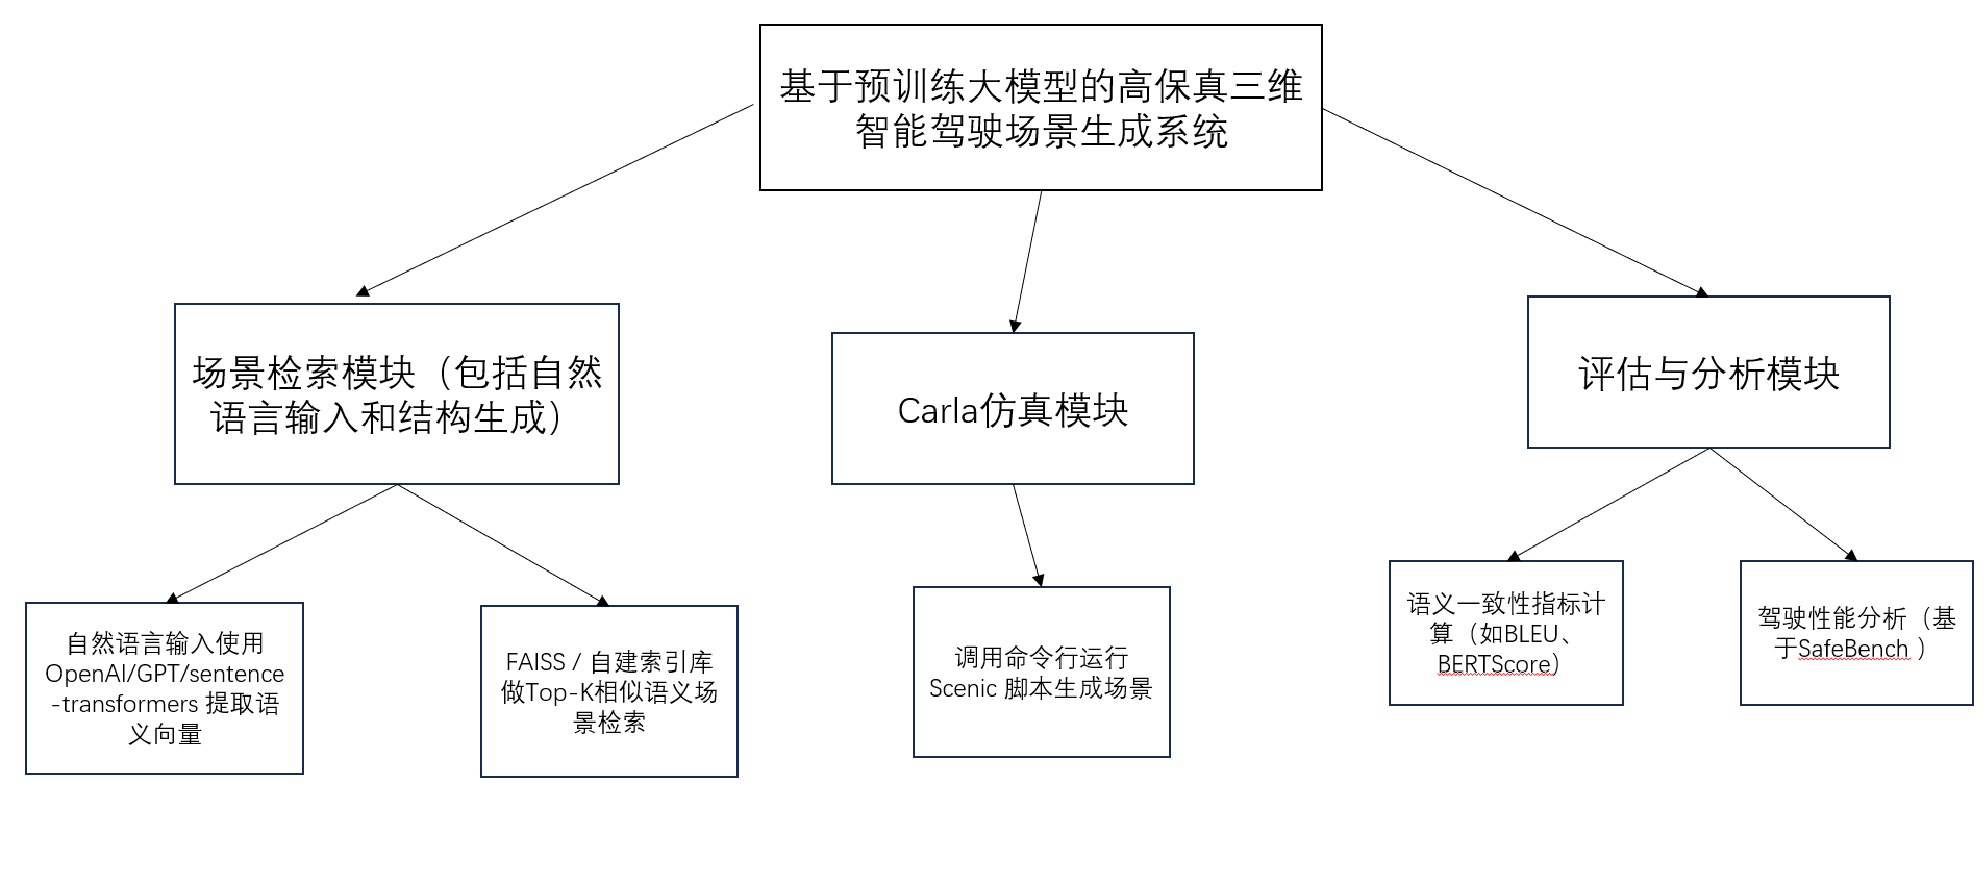
\includegraphics[width=1.0\textwidth]{images/系统架构图.pdf}
	\caption{系统架构}
	\label{fig:system-architecture}
\end{figure}
\subsection{自然语言输入模块}
介于需求分析,本系统实现了一个支持用户通过图形化界面或命令行形式输入文字交通场景描述的功能,提供友好的人机交互体验,确保用户能够方便地输入各种场景描述。为了实现这一目标,系统将采用 PyQt5 框架来构建图形化用户界面(GUI),以确保界面的简洁高效和跨平台兼容性。PyQt5 是一个功能强大的 Python GUI 框架,能够提供丰富的控件和灵活的布局选项,使得开发者可以设计出直观且易于使用的界面。

具体而言,系统将遵循极简主义设计原则,去除不必要的复杂元素,确保界面清晰、直观。用户可以通过简单的点击和输入操作完成场景描述的输入,而无需进行复杂的配置或学习。界面将提供清晰的提示信息和操作指引,帮助用户快速上手。同时,系统将优化输入流程,减少用户的操作步骤,例如通过自动填充常见信息、提供快捷输入选项等方式提高输入效率。此外,系统还将支持用户保存输入的场景描述,方便用户在后续使用中快速调用和修改。为了进一步提升用户体验,系统可以考虑引入智能提示功能,根据用户输入的内容实时推荐可能的场景描述选项,从而进一步提高输入的准确性和效率。总之,系统的自然语言场景输入功能将以简洁高效为核心,确保用户能够快速、准确地完成场景描述的输入,同时享受流畅的交互体验。
\subsection{结构生成模块}

结构生成模块是本系统连接语义理解与仿真执行的核心环节,主要任务是将语义检索得到的场景结构模板与自然语言输入内容融合,自动生成符合 Scenic 语法规范的结构化场景脚本(.scenic 文件)。该模块不仅要表达场景中的交通参与者及其属性,还需描述其行为逻辑、空间约束与触发机制,以保证场景具备完整性、可执行性与可控性。

在实际实现中,系统维护了一组参数化 Scenic 模板脚本,模板中预设了车辆、行人、道路、红绿灯等典型交通元素的结构框架与行为函数。例如用户输入“自车前方有行人突然横穿马路并停在车前”时,系统将匹配到“横穿-阻挡”场景模板,并结合输入语义为其中的参数插槽进行自动赋值,如横穿速度、横穿位置、停止距离等。
如图:
\begin{figure}[H]
	\centering
	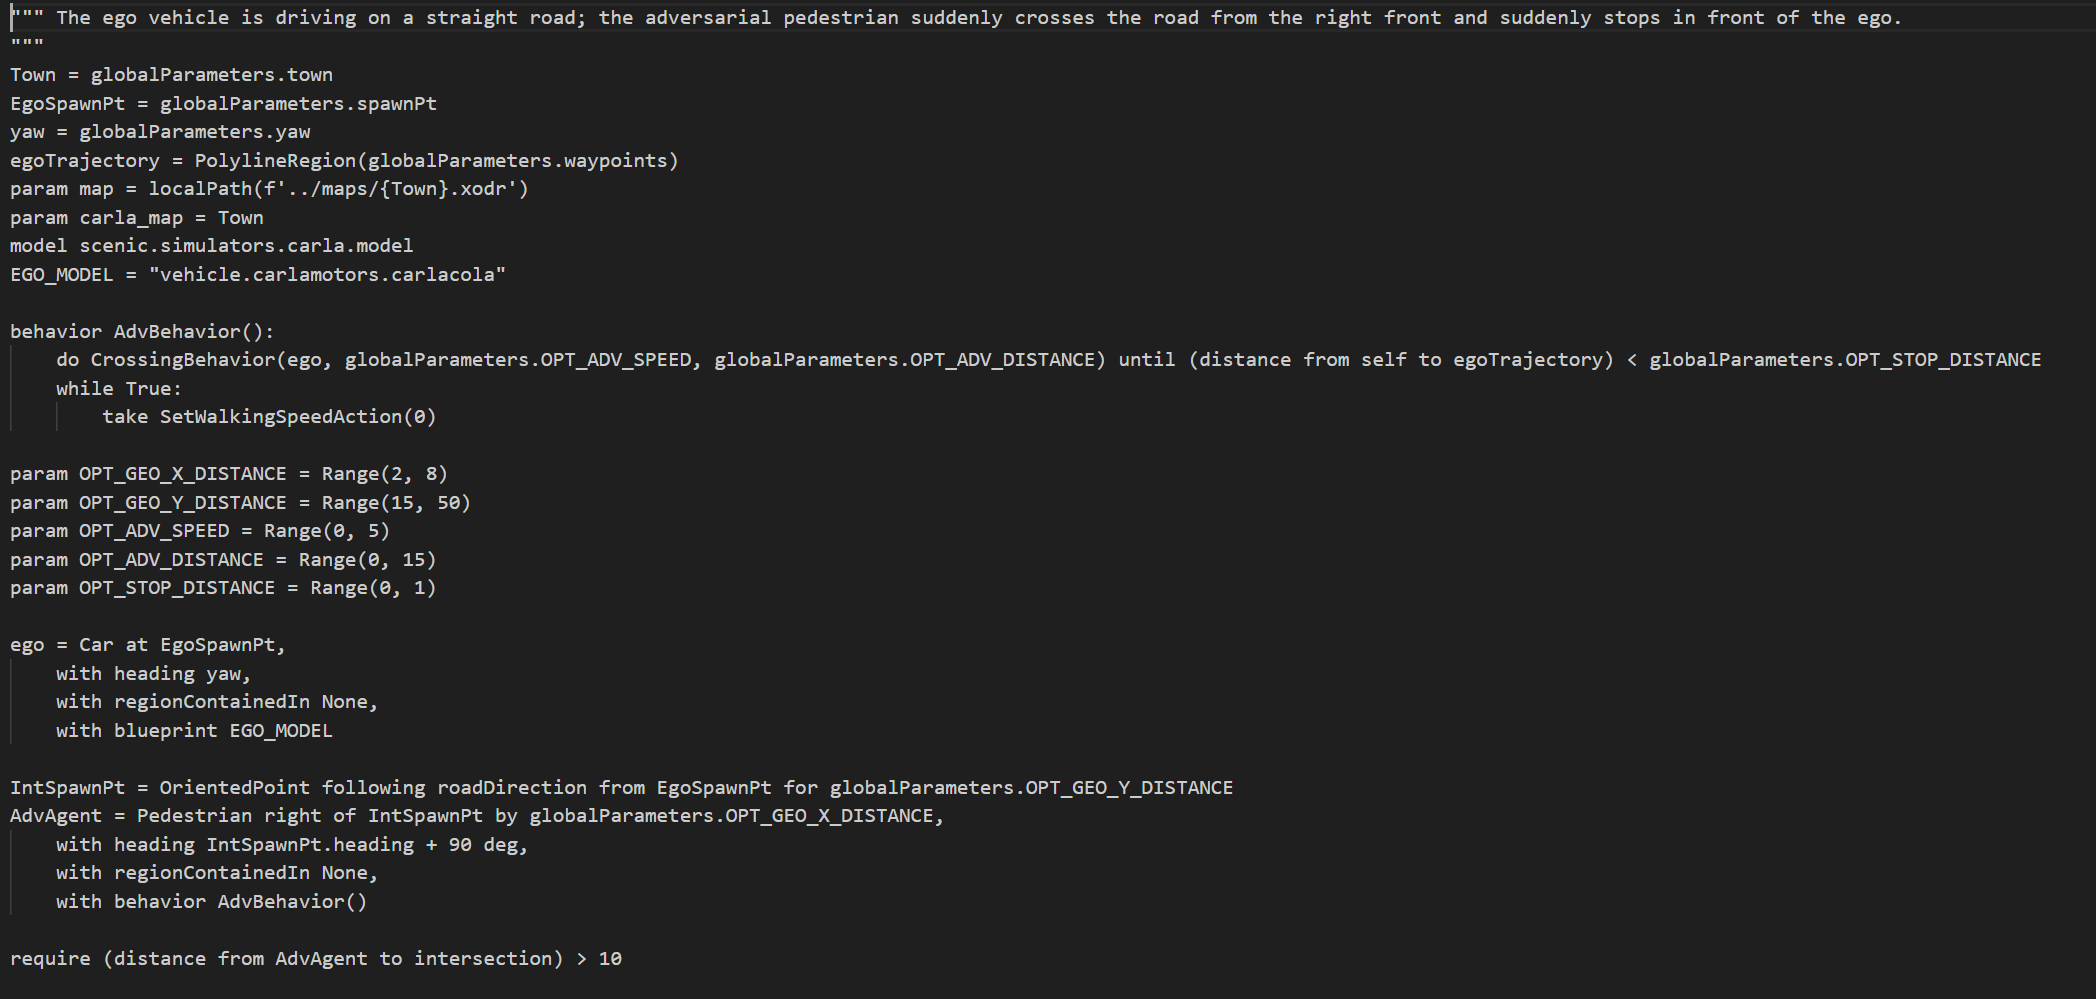
\includegraphics[width=1.0\textwidth]{images/scenic脚本示例1.png}
	\caption{Scenic 脚本示例}
	\label{fig:scenic-example1}
\end{figure}



 所示的 Scenic 示例脚本中,系统使用globalParameters模块中的可调参数如
 \texttt{OPT\_ADV\\ \_SPEED}、\texttt{OPT\_GEO\_X\_DISTANCE} 等控制行人的行为过程与生成位置,定义的行为函数 \texttt{AdvBehavior()}则包含了先横穿、再停下的动态行为建模。这些参数既可来自模板设定,也可从自然语言推理中注入,最终组合成具有时间逻辑与交互动态的场景剧本。

此外,结构生成模块支持在 Scenic 脚本中添加空间约束(如位于路口、靠右侧车道)、行为触发条件(如距离自车低于一定值停止)等语义规则。系统还支持为多个角色赋予不同行为序列,形成多主体互动的复杂场景。

最终生成的 Scenic 脚本将自动保存至 \texttt{scenario/scenario\_data/scenic\_d\\ata/} 目录下,供后续仿真调度模块调用执行,实现从自然语言到可执行场景的结构化表达闭环。

\subsection{carla仿真模块}

仿真调度模块是本系统实现自动驾驶场景可视化与执行验证的关键组件,主要负责将生成的 Scenic 脚本加载至 CARLA 仿真环境中,并进行仿真初始化、执行控制、传感器采集及过程管理等工作。该模块在本系统中由封装的 \texttt{ScenicRunnerDynamic} 类实现,调用 Scenic 官方提供的 \texttt{ScenicSimulator} 对生成脚本进行解析,并将其转化为可在 CARLA 中执行的场景实体。

在具体流程上,模块首先读取前一阶段生成的 .scenic 脚本,并通过 Scenic 编译器解析其中定义的交通参与者、位置、行为及约束条件。随后,系统基于 Carla Python API 建立仿真连接,配置运行地图、天气参数、物理步长(\texttt{fixed\_delta\_seconds})与同步模式等环境变量。系统默认使用 Carla 的同步模式进行控制,确保场景中各参与体的状态更新与传感器采集过程保持一致,提升仿真稳定性。

仿真执行过程中,系统自动创建交通参与体(如车辆、行人)并初始化其行为轨迹。若 Scenic 脚本中定义了行为函数(如“行人横穿并在自车前停止”),则系统会通过行为调度逻辑驱动对应实体执行脚本中预定义的动作。仿真过程中,模块还负责记录关键执行信息,包括仿真时间、对象轨迹、碰撞信息、交通信号状态等。同时,系统支持截图与视频保存功能,可自动截取仿真中间帧或生成仿真动画用于结果展示与评估。

该模块的运行过程为系统的“代码—仿真”环节提供了自动化调度能力,结合 CARLA 高保真的渲染与物理驱动能力,为自然语言驱动的场景生成系统提供了可视化反馈与执行验证平台,构成系统闭环中的关键一环。

\subsection{结果评估分析模块}

结果展示模块是系统用于输出仿真执行结果、可视化运行过程并辅助后续评估分析的重要组成部分。该模块负责接收来自仿真调度模块的运行数据与视觉信息,并以图像、视频和行为指标等多种形式呈现生成场景的实际效果。

在具体实现中,系统会在仿真执行过程中调用CARLA提供的图像传感器接口,自动截取关键帧并保存为静态图片,也可根据用户设置将整个仿真过程录制为视频文件,供展示与回放使用。同时,系统支持记录自车和关键参与体的轨迹坐标信息,形成时间序列形式的运动轨迹数据,可用于后续路径可视化或行车行为评估。

除了可视化结果,系统还内嵌了一套自动化的评估指标计算模块,包括碰撞率、交通违规频率、路线完成度、行为稳定性等多维度场景表现指标。运行结果会被整理为统一格式的评估表格,并可生成对应柱状图或折线图,帮助开发者从定量角度评估系统输出场景的质量与合理性。

此外,该模块还支持一键输出报告功能,可将自然语言输入、生成脚本、运行截图与关键指标整合为完整的实验记录文档,提升整体系统的可解释性与实验复现能力。通过结果展示模块,系统实现了从“自然语言生成 → 可视化仿真 → 结果评估”的完整闭环,确保生成场景不仅语义一致,而且具备运行合理性与仿真真实性。

